\chapter{Model Development Comparison Data}\label{ch:appClabel}

%\begin{table}[H]
%\centering
%	\caption{Models.}
%	\begin{tabular}{ l  c }
%	Model1 -\tikzcircle[pink, fill=pink]{3pt}- &
%	(Their simpleLSTM Model)\\
%	Model2 -\tikzcircle[red, fill=red]{3pt}- &
%	(Our simpleLSTM Model)\\
%	Model3 -\tikzcircle[turquoise, fill=turquoise]{3pt}- &
%	(Our BiRNN Model)\\
%	\end{tabular}
%	\label{tab:3_models}
%\end{table}
%\begin{table}[H]
%\centering
%    \caption{Parameter values of the three model.}
%    \begin{tabular}{| l | c | c | c | c |} 
%    \hline
%        Parameters & 
%        Model1 -\tikzcircle[pink, fill=pink]{3pt}- &
%        Model2 -\tikzcircle[red, fill=red]{3pt}- &
%        Model3 -\tikzcircle[turquoise, fill=turquoise]{3pt}-\\
%    \hline
%        Batch Size & 
%        50 \hfill 20 \hfill 20 & 
%        50 \hfill 20 \hfill 20 & 
%        50 \hfill 20 \hfill 20 \\
%    \hline
%        Dropout & 
%        0.05 & 0.05 & 0.05 \\
%    \hline
%        Learning Rate & 
%        0.001 & 0.001 & 0.001 \\ 
%    \hline
%    \end{tabular}
%    \label{tab:3models_tab}
%\end{table}

\begin{table}[H]
\begin{minipage}{0.5\textwidth}
\centering
	\caption{Test error rate results.}
	\begin{tabular}{| l | c | c | c |}
	\hline
	Models & Value & Epoch & Duration \\
	\hline
	Model1 -\tikzcircle[pink, fill=pink]{3pt}- &
	0.200 & 25.00 & 0s\\
	\hline
	Model2 -\tikzcircle[red, fill=red]{3pt}- &
	0.080 & 25.00 & 0s\\
	\hline
	Model3 -\tikzcircle[turquoise, fill=turquoise]{3pt}- &
	0.000 & 25.00 & 0s\\
	\hline
	\end{tabular}
\end{minipage}
\begin{minipage}[c]{0.5\textwidth}
\centering
	\caption{Training error rate results.}
	\begin{tabular}{| l | c | c | c |}
	\hline
	Models & Value & Epoch & Duration \\
	\hline
	Model1 -\tikzcircle[pink, fill=pink]{3pt}- &
	2.0887e-3 & 24.00 & 7m 46s\\
	\hline
	Model2 -\tikzcircle[red, fill=red]{3pt}- &
	5.1642e-3 & 24.00 & 9m 47s\\
	\hline
	Model3 -\tikzcircle[turquoise, fill=turquoise]{3pt}- &
	0.000 & 24.00 & 12m 50s\\
	\hline
	\end{tabular}
\end{minipage}%
\end{table}
\begin{table}[H]
\begin{minipage}{0.52\textwidth}
\centering
	\caption{Validation error rate results.}
	\begin{tabular}{| l | c | c | c |}
	\hline
	Models & Value & Epoch & Duration \\
	\hline
	Model1 -\tikzcircle[pink, fill=pink]{3pt}- &
	0.1669 & 23.00 & 7m 9s\\
	\hline
	Model2 -\tikzcircle[red, fill=red]{3pt}- &
	0.2030 & 23.00 & 9m 8s\\
	\hline
	Model3 -\tikzcircle[turquoise, fill=turquoise]{3pt}- &
	0.01398 & 23.00 & 11m 49s\\
	\hline
	\end{tabular}
\end{minipage}
\begin{minipage}[c]{0.5\textwidth}
\centering
	\caption{Training average loss results.}
	\begin{tabular}{| l | c | c | c |}
	\hline
	Models & Value & Epoch & Duration \\
	\hline
	Model1 -\tikzcircle[pink, fill=pink]{3pt}- &
	0.04573 & 24.00 & 7m 46s\\
	\hline
	Model2 -\tikzcircle[red, fill=red]{3pt}- &
	0.1608 & 24.00 & 9m 47s\\
	\hline
	Model3 -\tikzcircle[turquoise, fill=turquoise]{3pt}- &
	1.2939e-3 & 24.00 & 12m 50s\\
	\hline
	\end{tabular}
\end{minipage}%
\end{table}
\begin{figure}[H]
    \centering
    \begin{minipage}{0.5\textwidth}
        \centering
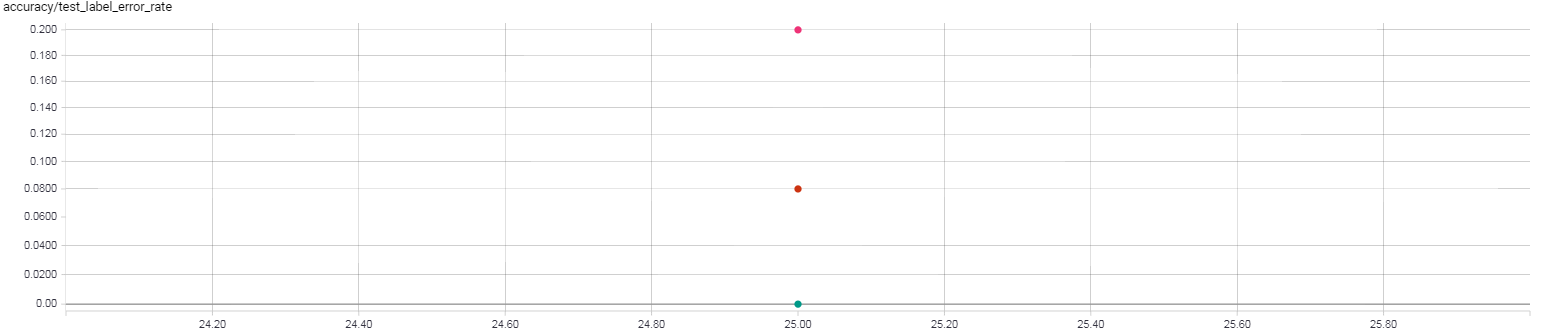
\includegraphics[width=3\textwidth, angle=90]		
	{model_development/3models_comparison/test_error_rate_3models}
        \caption{Test error rate.}
    \end{minipage}\hfill
    \begin{minipage}{0.5\textwidth}
        \centering
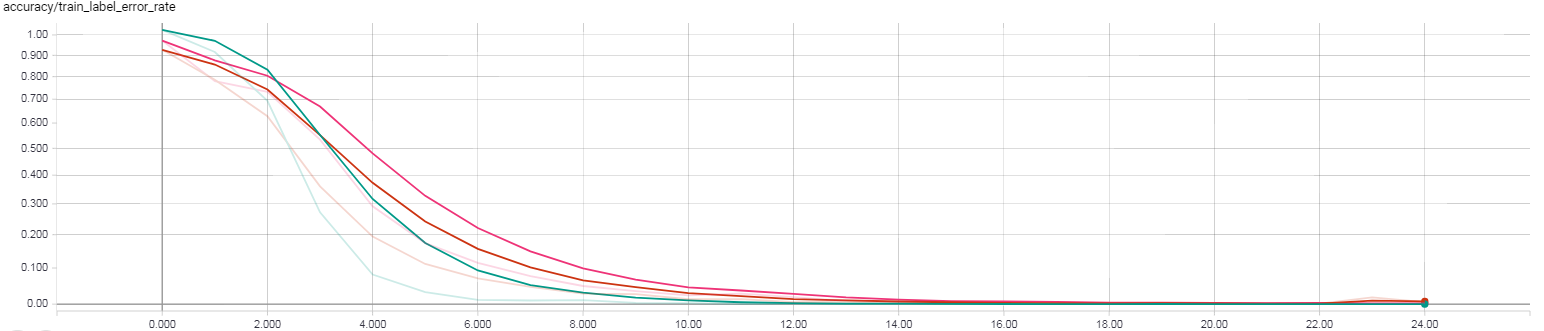
\includegraphics[width=3\textwidth, angle=90]	
	{model_development/3models_comparison/train_error_rate_3models}
        \caption{Training error rate.}
    \end{minipage}
\end{figure}
\begin{figure}[H]
    \centering
    \begin{minipage}{0.5\textwidth}
        \centering
	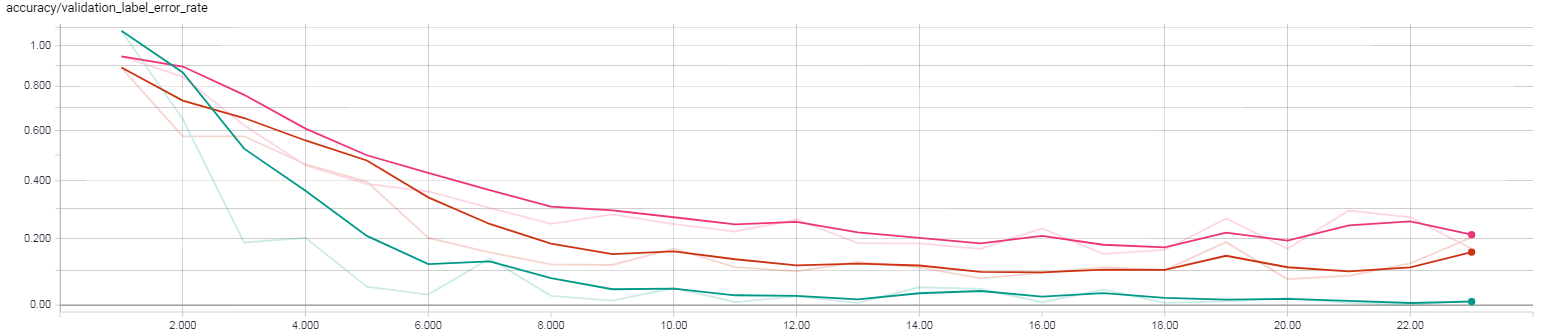
\includegraphics[width=3\textwidth, angle=90]		
	{model_development/3models_comparison/validation_error_rate_3models}
        \caption{Validation error rate.}
    \end{minipage}\hfill
    \begin{minipage}{0.5\textwidth}
        \centering
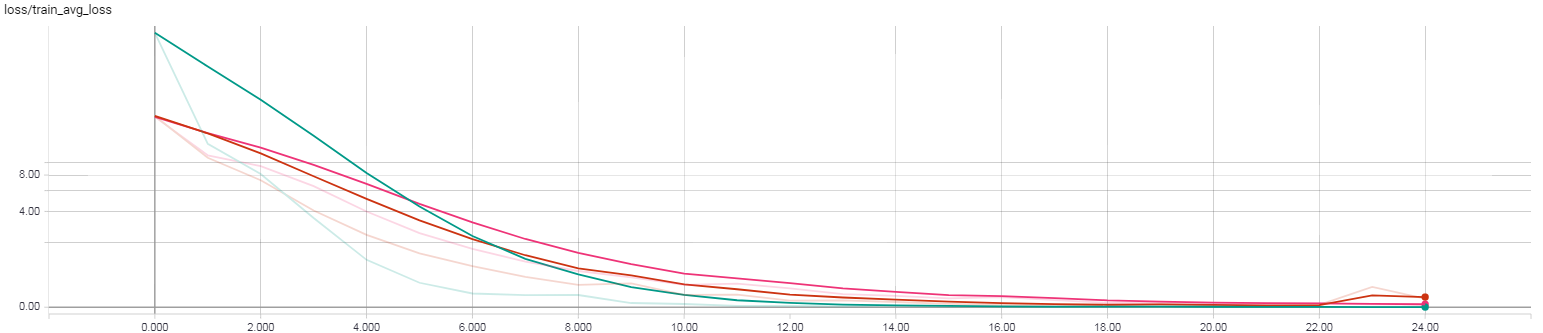
\includegraphics[width=3\textwidth, angle=90]		
	{model_development/3models_comparison/train_avg_loss_3models}
        \caption{Training average loss.}
    \end{minipage}
\end{figure}

%\begin{figure}[H]
%	\centering
%	\includegraphics[width=\textwidth]		
%	{model_development/3models_comparison/test_error_rate_3models}
%	\caption{Test error rate.}
%\end{figure}
%\begin{figure}[H]
%	\centering
%	\includegraphics[width=\textwidth]		
%	{model_development/3models_comparison/train_error_rate_3models}
%	\caption{Training error rate.}
%\end{figure}
%\begin{figure}[H]
%	\centering
%	\includegraphics[width=\textwidth]		
%	{model_development/3models_comparison/validation_error_rate_3models}
%	\caption{Validation error rate.}
%\end{figure}
%\begin{figure}[H]
%	\centering
%	\includegraphics[width=\textwidth]		
%	{model_development/3models_comparison/train_avg_loss_3models}
%	\caption{Training average loss.}
%\end{figure}
%\begin{table}[H]
%\centering
%	\caption{Test error rate results.}
%	\begin{tabular}{| l | c | c | c |}
%	\hline
%	Models & Value & Epoch & Duration \\
%	\hline
%	Model1 -\tikzcircle[pink, fill=pink]{3pt}- &
%	0.200 & 25.00 & 0s\\
%	\hline
%	Model2 -\tikzcircle[red, fill=red]{3pt}- &
%	0.080 & 25.00 & 0s\\
%	\hline
%	Model3 -\tikzcircle[turquoise, fill=turquoise]{3pt}- &
%	0.000 & 25.00 & 0s\\
%	\hline
%	\end{tabular}
%\end{table}
%\begin{table}[H]
%\centering
%	\caption{Training error rate results.}
%	\begin{tabular}{| l | c | c | c |}
%	\hline
%	Models & Value & Epoch & Duration \\
%	\hline
%	Model1 -\tikzcircle[pink, fill=pink]{3pt}- &
%	2.0887e-3 & 24.00 & 7m 46s\\
%	\hline
%	Model2 -\tikzcircle[red, fill=red]{3pt}- &
%	5.1642e-3 & 24.00 & 9m 47s\\
%	\hline
%	Model3 -\tikzcircle[turquoise, fill=turquoise]{3pt}- &
%	0.000 & 24.00 & 12m 50s\\
%	\hline
%	\end{tabular}
%\end{table}
%\begin{table}[H]
%\centering
%	\caption{Validation error rate results.}
%	\begin{tabular}{| l | c | c | c |}
%	\hline
%	Models & Value & Epoch & Duration \\
%	\hline
%	Model1 -\tikzcircle[pink, fill=pink]{3pt}- &
%	0.1669 & 23.00 & 7m 9s\\
%	\hline
%	Model2 -\tikzcircle[red, fill=red]{3pt}- &
%	0.2030 & 23.00 & 9m 8s\\
%	\hline
%	Model3 -\tikzcircle[turquoise, fill=turquoise]{3pt}- &
%	0.01398 & 23.00 & 11m 49s\\
%	\hline
%	\end{tabular}
%\end{table}
%\begin{table}[H]
%\centering
%	\caption{Training average loss results.}
%	\begin{tabular}{| l | c | c | c |}
%	\hline
%	Models & Value & Epoch & Duration \\
%	\hline
%	Model1 -\tikzcircle[pink, fill=pink]{3pt}- &
%	0.04573 & 24.00 & 7m 46s\\
%	\hline
%	Model2 -\tikzcircle[red, fill=red]{3pt}- &
%	0.1608 & 24.00 & 9m 47s\\
%	\hline
%	Model3 -\tikzcircle[turquoise, fill=turquoise]{3pt}- &
%	1.2939e-3 & 24.00 & 12m 50s\\
%	\hline
%	\end{tabular}
%\end{table}

\begin{figure}[H]
	\centering
	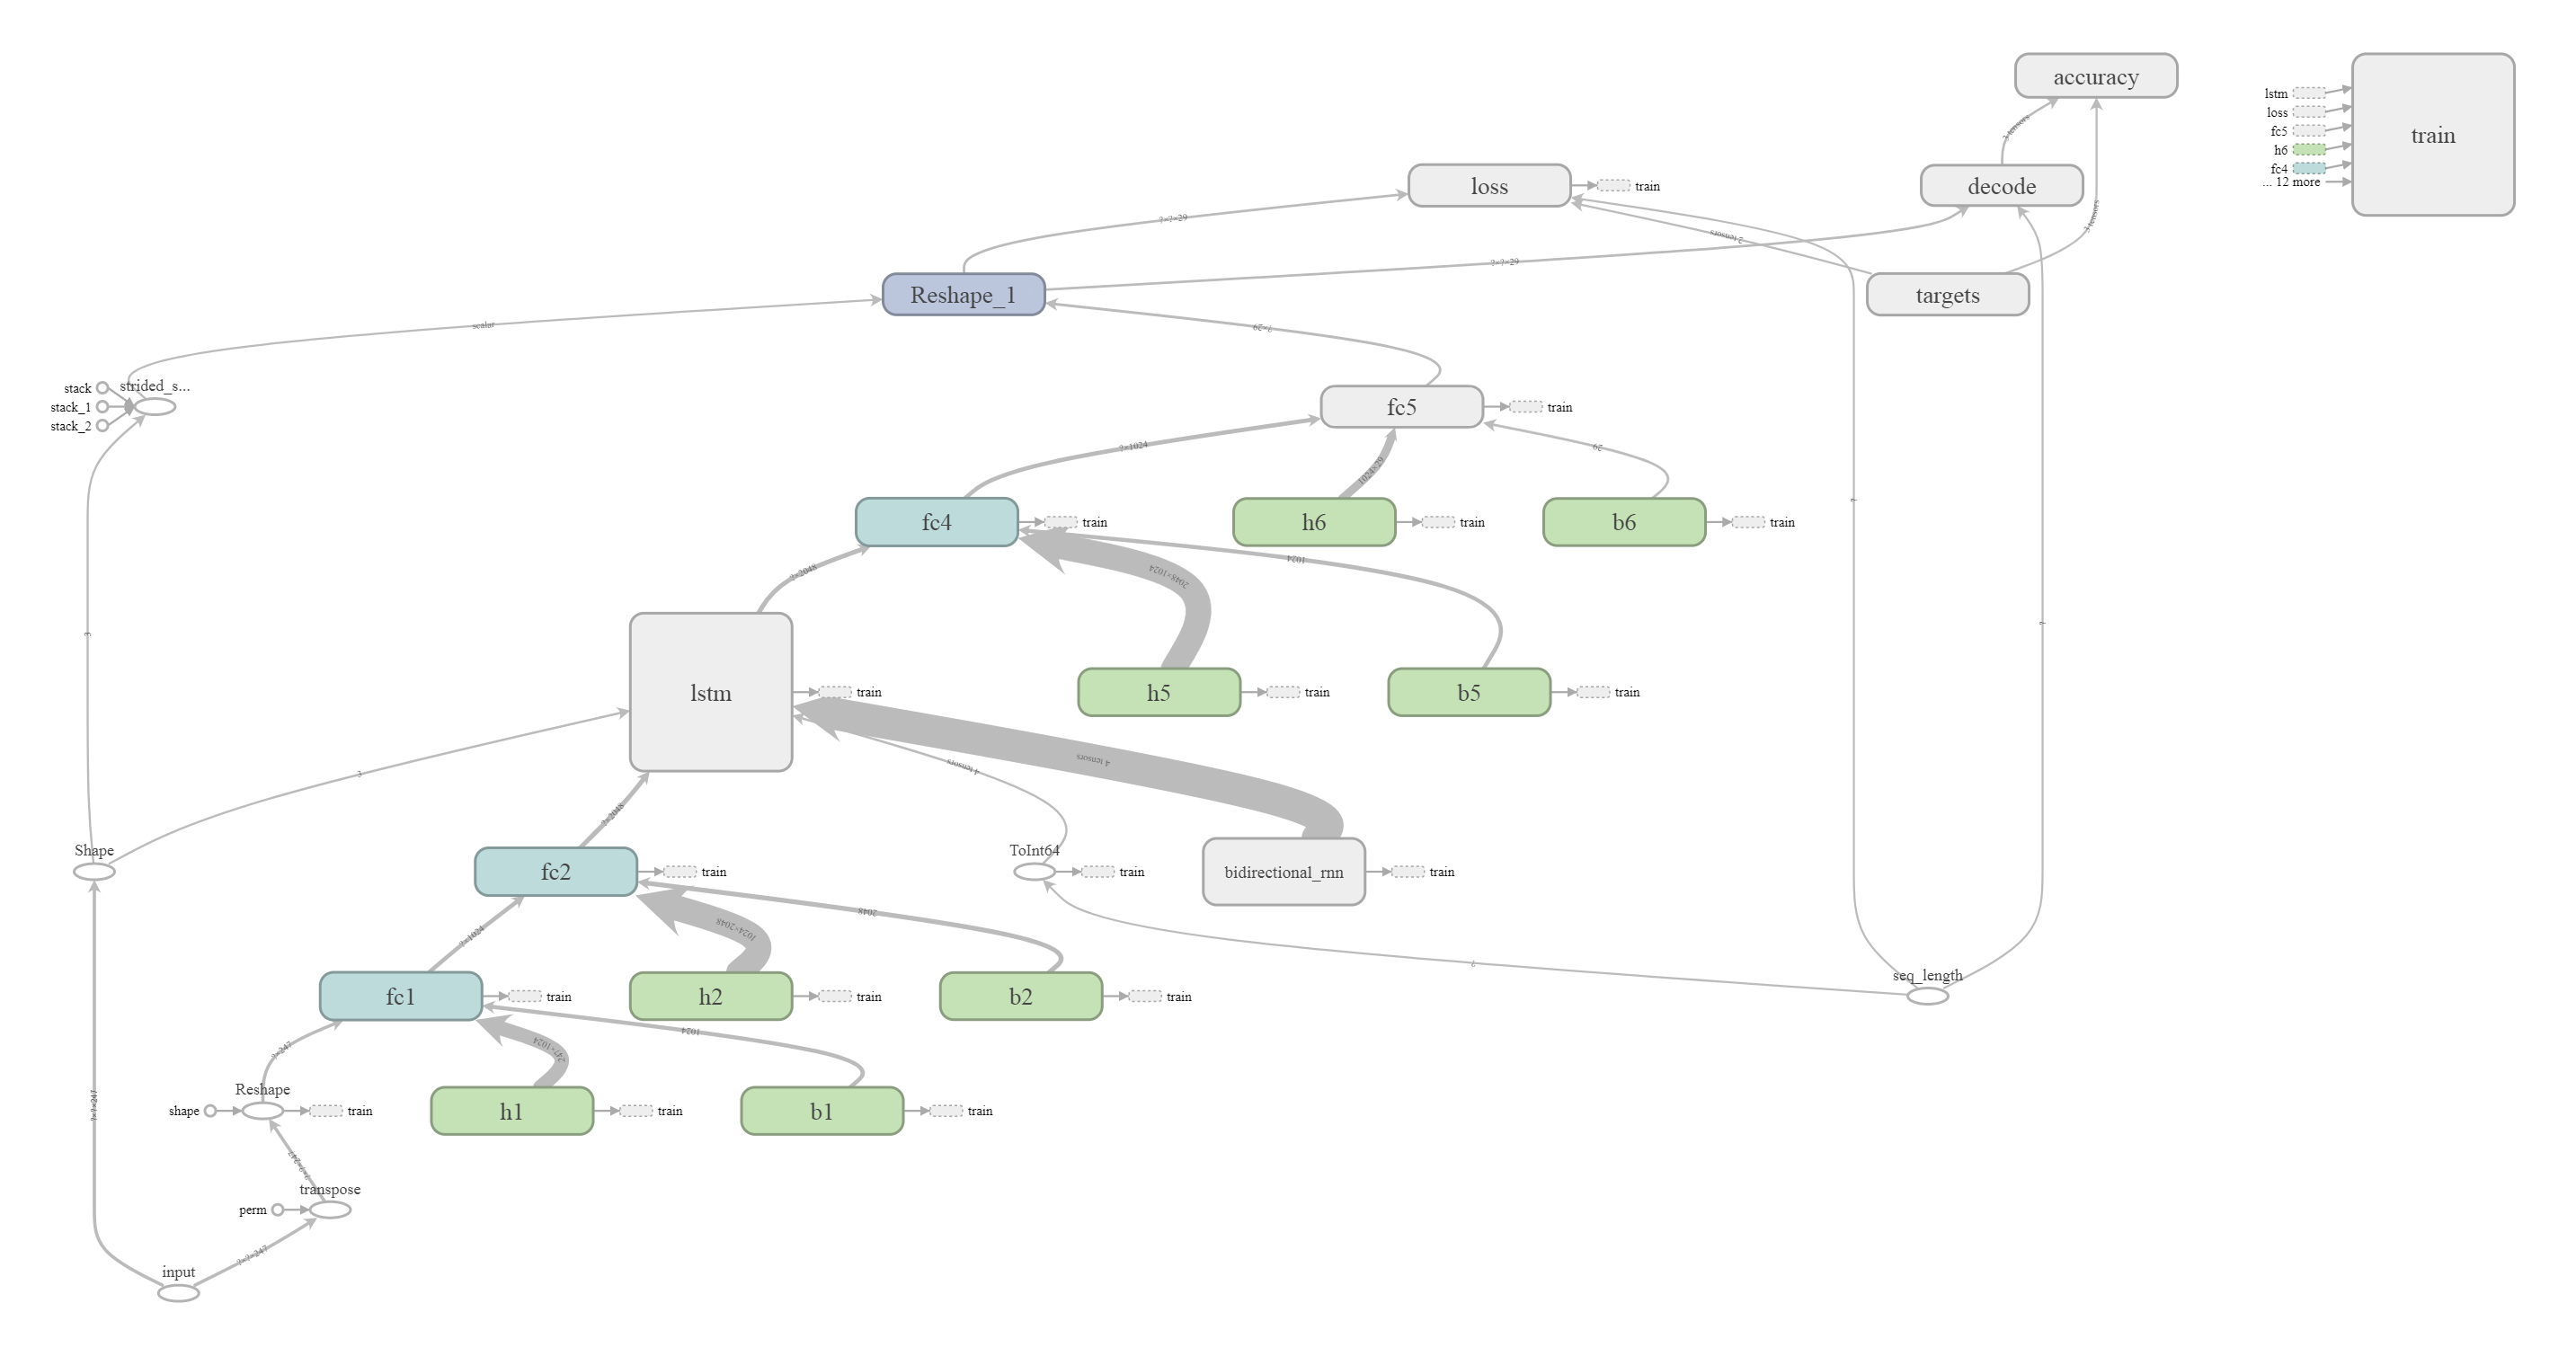
\includegraphics[width=1.6\textwidth, angle=90]		
	{model_development/birnn_v2_graph}
	\caption{Our BiRNN model graph.}
\end{figure}
